\documentclass[8pt]{beamer}
\usepackage[nobglogo]{beamerthemedmi-owled}
\usepackage[utf8x]{inputenc}
\usepackage{default}
\usepackage{url}
\usepackage{verbatim}
\usepackage{graphicx}
\usepackage{mathrsfs}
\usepackage{dl}
\usepackage{mls}
%\usepackage{listings}


\mode<presentation>
{
  \usetheme{dmi-owled}
  %\usetheme{Warsaw}
  % or ...

  \setbeamercovered{transparent}
  % or whatever (possibly just delete it)
}

\title{Web Reasoning 2015/2016\\
Lezione 1}

\author{Cristiano Longo\\ 
{\small{longo@dmi.unict.it}}}



\date{Universit\`a di Catania, TODO 2015}
\newcommand{\urlsingle}[1]{{\small {\center {\url{#1}}}}}
\begin{document}
\maketitle
\setcounter{tocdepth}{1}

\section{Introduzione}

\begin{frame}
\frametitle{World Wide Web - nascita}
\begin{quote}
Imagine, then, the references in this document all being associated with 
the network address of the thing to which they referred, so that while 
reading this document you could skip to them with a click of the mouse.
\end{quote}
\vspace{\baselineskip}
\emph{Semantic Web Roadmap}, Tim Berners-Lee, 1989.
\vspace{\baselineskip}

\uncover<2->{
Nel 1993 il CERN rilascer\`a di pubblico dominio i primi software per il
world wide web, tra cui il primo browser chiamato per l'appunto \emph{World
Wide Web}.\footnote{\url{http://home.cern/topics/birth-web}} 
}
\end{frame}

\begin{frame}
\frametitle{World Wide Web - definizione}
\begin{quote}
The World Wide Web (WWW, or simply Web) is an information space in which
the items of interest, referred to as resources, are identified by global
identifiers called Uniform Resource Identifiers (URI).
\end{quote}
\vspace{\baselineskip}
\emph{Architecture of the World Wide Web, Volume
I}\footnote{\url{https://www.w3.org/TR/webarch/}}
\vspace{\baselineskip}

\uncover<2->{
Le prime specifiche rilasciate furono:
\begin{itemize}
  \item Uniform Resource Locators (URLs),
  \item Hypertext Transfer Protocol (HTTP),
  \item Hypertext Markup Language (HTML).
\end{itemize}
}
\end{frame}

\begin{frame}
\frametitle{Limiti del World Wide Web (1/4)}
\begin{quote}
The Web was designed as an information space, with the goal that it should be 
useful not only for human-human communication, but also that machines would be
able to participate and help. One of the major obstacles to this has been the
fact \textbf{that most information on the Web is designed for human consumption}, and 
even if it was derived from a database with well defined meanings (in at least 
some terms) for its columns, that \textbf{the structure of the data is not evident to 
a robot browsing the web.}  
\end{quote}
\vspace{\baselineskip}
\emph{Semantic Web Roadmap}, Tim Berners-Lee, 1998.
\end{frame}

\begin{frame}
\frametitle{Limiti del World Wide Web (2/4)}
Alcuni problemi nell'interpretazione di testi derivano da:
\begin{description}
 \item[Lingue Differenti] e.g. $Parigi$ e $Paris$ possono indicare la stessa citt\`a.
 \item[Omonimie] e.g. esistono svariate citt\`a chiamate 
 \emph{Paris} nel mondo (Arkansas, Idaho, Illinois, Kentucky,
 Maine, Michigan, Missouri, New York, \ldots);
\end{description}
\end{frame}

\begin{frame}
\frametitle{Limiti del World Wide Web (3/4)}

La situazione si complica in presenza di contenuti multimediali.

\begin{figure}
    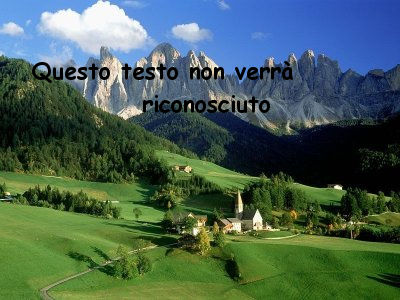
\includegraphics[width=250px]{unrecognizable.jpg} 
\end{figure}
\end{frame}

\begin{frame}
\frametitle{Limiti del World Wide Web (4/4)}
Come conseguenza, spesso \`e impossibile eseguire su web ricerce 
\emph{complesse} ottenendo risultati accurati. Ad esempio, cercando sul web
\emph{``Federico II places''} non si ottengono risultati in prima pagina su 
Federico II, ma solo sull'omonima universit\`a:
  
  \begin{small}
    \begin{enumerate}
   \item Universit\`a degli Studi di Napoli "Federico II" | OPEN Places
   \item AOU - Policlinico "Federico II" - Napoli, Italy - Hospital | Facebook
   \item Federico II Ingegneria Via Claudio - College and University | Facebook
   \item MARIA CATERINA FONTE - www.docenti.unina.it
  \end{enumerate}
  \end{small}
\end{frame}

\begin{frame}
\frametitle{Il Web Semantico (1/2)}
\begin{quote}
[\ldots] the Semantic Web approach instead develops languages for expressing
information in a machine processable form. 
\end{quote}
\emph{Semantic Web Roadmap}, Tim Berners-Lee, 1998.

\begin{figure}
    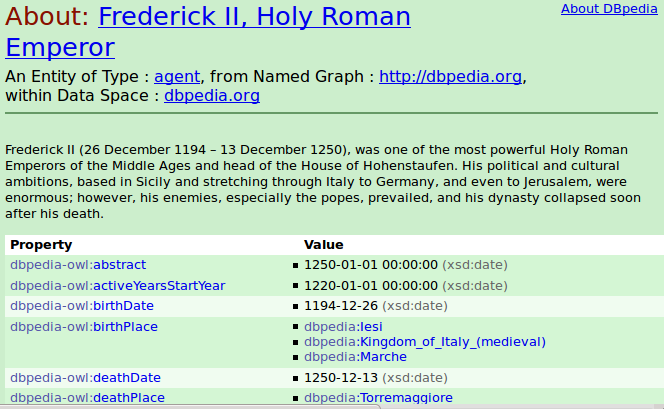
\includegraphics[width=250px]{federicoII_dbpedia.png} 
    \caption{Federico II su dbpedia.org}
\end{figure}
\end{frame}

\begin{frame}
\frametitle{Il Web Semantico (2/2)}

 Il \emph{Web Semantico} nasce per associare informazioni 
 \emph{strutturate} alle pagine web, che solitamente sono
 composte da testo libero.\footnote{Vedi \emph{Semantic Web Roadmap}, Tim Berners-Lee, 1998.}
 \vspace{\baselineskip}

\uncover<2->{
I \emph{linguaggi di rappresentazione} usati nel Web semantico 
hanno una \emph{sintassi rigorosa} e sono dotati di una \emph{semantica formale}.
\vspace{\baselineskip}
}

\uncover<3->{
Questo rende possibile effettuare interrogazioni complesse 
ottenendo dei risultati precisi anche se a volte parziali:

\begin{center}
Q = “Luoghi di nascita di Federico II e dei suoi parenti stretti” . 
\end{center}
}
\end{frame}

\begin{frame}
\frametitle{Linked Data (1/3)}
\begin{quote}
The Semantic Web is a web of data, in some ways like a global database.
\end{quote}
\small{\emph{Semantic Web Roadmap}, Tim Berners-Lee, 1998.}
\begin{figure}
    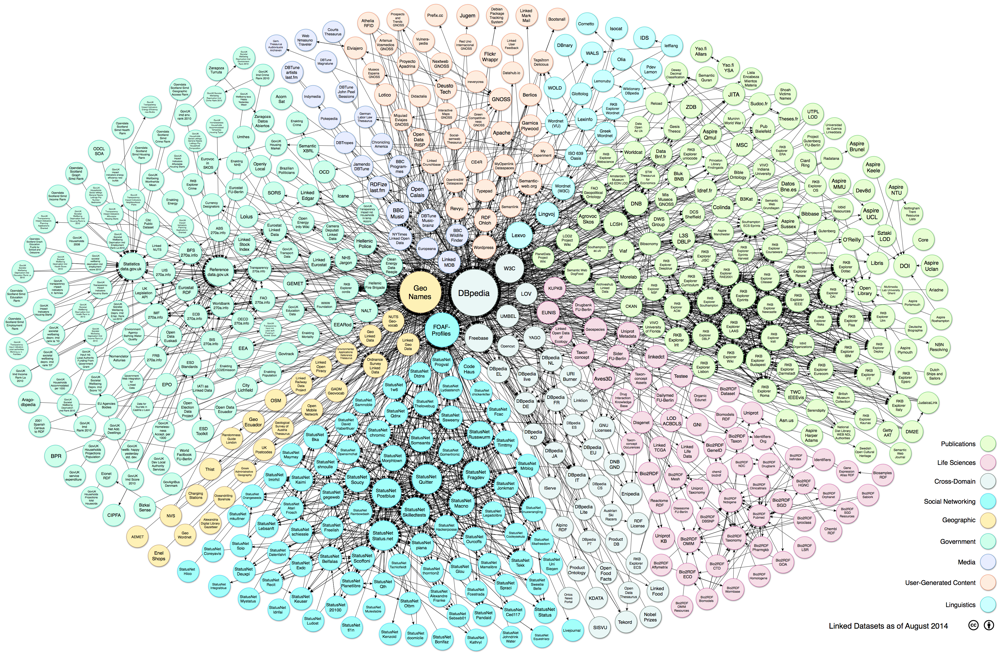
\includegraphics[width=250px]{lod-cloud_colored_1000px.png} 
    \caption{Linked Open Data Cloud}
\end{figure}
\end{frame}

\begin{frame}
\frametitle{Linked Data (2/3)}
Nel \emph{Linked Open Data Cloud} sono presenti 365
\emph{ontologie}(fonte \url{http://stats.lod2.eu/}).\footnote{spesso ci si riferisce alle ontologie usando il
termine \emph{dataset}.}
\vspace{\baselineskip}

Alcune di queste sono:
\begin{itemize}
 \item \emph{DBPedia} (\url{dbpedia.org}) corrispondente a \url{wikipedia.org};
 \item \emph{Linked Movie Database} (\url{http://linkedmdb.org/}) controparte sul Web Semantico di \emph{Internet Movie Database} 
 (\url{http://www.imdb.com/});
 \item \emph{Linked GeoData} (\url{http://linkedgeodata.org}) 
  contiene i dati di \emph{OpenStreetMap} (\url{http://www.openstreetmap.org/});
  \item \emph{AGROVOC} (\url{http://aims.fao.org/agrovoc}) \`e l'ontologia della
  FAO (\url{http://fao.org});
  \item \emph{Europeana} (\url{http://pro.europeana.eu/linked-open-data}) contiene dati su beni culturali e tradizioni Europee. 
\end{itemize}
\end{frame}

\begin{frame}
\frametitle{Linked Data (3/3)}
\`E possibile effettuare interrogazioni che coinvolgano diverse
ontologie (anche eterogenee).
\vspace{\baselineskip}

Ad esempio, la seguente query pu\`o essere eseguita
interrogando una ontologia contenente dati storici ed una 
sulle strutture ricettive:


\begin{center}
Q = “Strutture ricettive nei luoghi di nascita di Federico II e dei suoi parenti stretti.”
\end{center}
\end{frame}


\end{document}